\documentclass{beamer}
%\usepackage{colortbl}
\usepackage[latin1]{inputenc}
\usepackage{comment}
%\usetheme{Warsaw}
\usetheme{Frankfurt}
%\usecolortheme{dove}
\usefonttheme{professionalfonts} 

\usepackage[absolute,overlay]{textpos} 
\usepackage{booktabs}
\usepackage{color}
\usepackage{threeparttable}
\usepackage{multirow}
%\usepackage[table]{xcolor}
%\definecolor{tableShade}{HTML}{F1F5FA}
\usepackage[normalem]{ulem}


\title[Epistasis and eQTL]{Epistasis in eQTL studies}
\author{Gibran Hemani}
\date{\today}
\begin{document}

\AtBeginSection[]
{
  \begin{frame}<beamer>
    \frametitle{Outline}
    \tableofcontents[currentsection,currentsubsection]
  \end{frame}
}

\begin{frame}
\titlepage
\end{frame}

\begin{comment}


____________intro

what is a gwas?
mixed success. missing heritability
endophenotypes

epistasis
- define epistasis
- how to search (two stages, two dimensions, mention epiGPU)

can epistasis maintain additive variance?
- yes.
- it actually maintains non-additive variation much more
- how do we search for epistasis?

____________conclusions

is the observation of additive variance an illusion?
have we misused occam's razor?
here is the paradox:
if you can measure additive genetic variance, search for non-additive variance

____________acknowledgements


\end{comment}



%%%%%%%%%%%%%%%%%%%%%%%%%%%%%%%%

\section{Intro to epistasis}
\subsection{}

%%%%%%%%%%%%%%%%%%%%%%%%%%%%%%%%



\begin{frame}{Genome wide association studies}
	\begin{center}
		\includegraphics[height=7cm]{gwas.jpg} \\
		{\tiny Wang 2009}
	\end{center}
\end{frame}

\begin{frame}{Additive variance paradigm}
	\begin{equation}
		V_{phenotype} = V_{{Additive} {Genetic}} + V_{{Everything} {Else}} \nonumber
	\end{equation}
	\begin{itemize}
		\item Discover common mutations that affect phenotypes
		\item Uncover genes and structural elements involved in disease
		\item Understand the architecture of natural genetic variation
	\end{itemize}
\end{frame}


\begin{frame}{Endophenotypes}
	\begin{center}
		\includegraphics[height=7cm]{broadgp.png}
	\end{center}
\end{frame}

\begin{frame}{Epistasis}
	\begin{center}
		\includegraphics[width=8cm]{gpmaps2.pdf}
	\end{center}
	\begin{definition}
		The effect on the phenotype caused by locus A depends on the genotype at locus B
	\end{definition}
\end{frame}

\begin{frame}{2D GWAS}
	\begin{center}
		\includegraphics[height=7cm]{2dscan.png}
	\end{center}
\end{frame}



%%%%%%%%%%%%%%%%%%%%%%%%%%%%%%%%

\section{Computational solutions}
\subsection{}

%%%%%%%%%%%%%%%%%%%%%%%%%%%%%%%%



\begin{frame}{The problem}
	\begin{block}{Number of interactions}
		\begin{equation}
			n(n-1) / 2 \nonumber
		\end{equation}
		500000 SNPs $\rightarrow$ 125 billion interactions
	\end{block}

	\begin{table}[ht]
		\begin{center}
			\begin{tabular}{lrl}
				\hline
				Software & Tests per second & Run time \\ 
				\hline
				PLINK & 5000 & 3 years \\ 
				Optimised CPU code & 125000 & 6 weeks \\ 
				Parallelised on 8-core CPU & 1000000 & 5 days \\ 
			   \hline
			\end{tabular}
		\end{center}
	\end{table}
\end{frame}


\begin{frame}{CPU limits}
	\begin{center}
		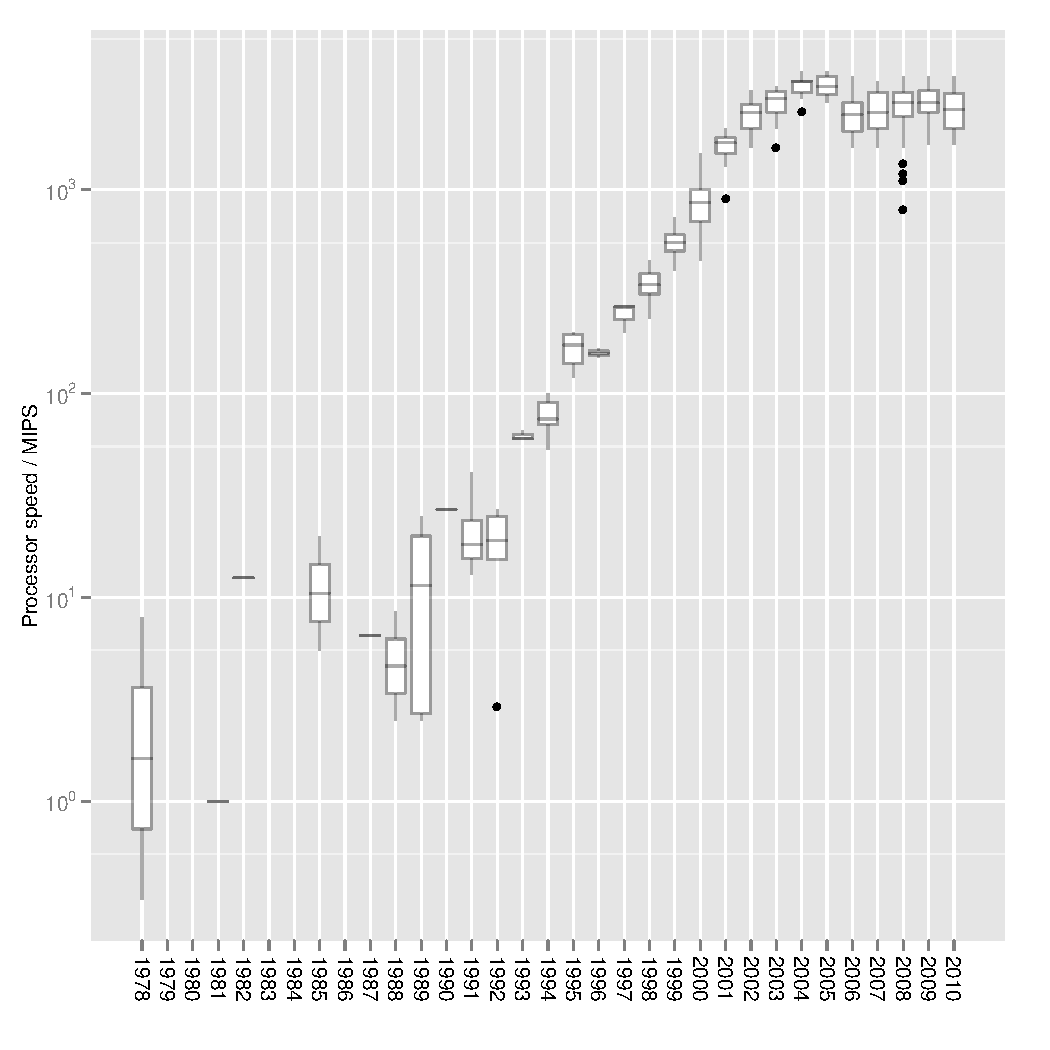
\includegraphics[height=7cm]{clockspeed.pdf}
	\end{center}
\end{frame}

\begin{frame}{Failed targets}
	\begin{center}
		\includegraphics[height=7cm]{clockrates.png}
	\end{center}
\end{frame}


\begin{frame}{Graphics Cards}
	\begin{center}
		\includegraphics[width=10cm]{gtx580}
	\end{center}
\end{frame}



\begin{frame}{GPU speeds}
	\begin{center}
		\includegraphics[height=7cm]{gpuoptimisation.pdf}
	\end{center}
\end{frame}

\begin{frame}{epiGPU}	
	\begin{block}{Download}
		{\tt sourceforge.net/projects/epigpu/}
	\end{block}
	\begin{itemize}
		\item Free
		\item Open source
		\item Windows, Mac, Linux
		\item NVIDIA and ATI graphics cards
	\end{itemize}
\end{frame}



%%%%%%%%%%%%%%%%%%%%%%%%%%%%%%%%

\section{2D eQTL}
\subsection{}

%%%%%%%%%%%%%%%%%%%%%%%%%%%%%%%%



\begin{frame}{Are epistatic effects controlling gene expression?}
	\begin{block}{Study design}
		\begin{itemize}
			\item 846 healthy Australian adults
			\item 546,192 SNPs
			\item 5380 gene expression probes from whole blood
		\end{itemize}
	\end{block}
	\begin{block}{Task}
		Perform exhaustive search for 2 locus epistasis for each probe
	\end{block}
	\begin{itemize}
		\item Parallelise search across 100x GPU cluster
		\item 802,494,666,067,680 tests in total...
	\end{itemize}
\end{frame}

\begin{frame}{Thresholds}

	\begin{block}{Bonferroni correction}
		\textbf{Adjust p-value by the number of tests that are being performed}\\
		We want the probability of there being a false positive at the end of the experiment to be limited to 0.05
	\end{block}
	\begin{equation}
		-\log_{10}\left ( \frac{0.05}{802\times10^{14}} \right) \approx 16.5 \nonumber
	\end{equation}
	\begin{block}{The curse of dimensionality}
		As the dimensionality of the search increases the background noise drowns out all real biological signals
	\end{block}
\end{frame}


\begin{frame}{Linkage disequilibrium}
	\begin{center}
		\includegraphics[width=8cm]{ld.png}
	\end{center}
	\begin{itemize}
		\item SNPs are correlated $\rightarrow$ tests are not independent
		\item Bonferroni correction is overly stringent
		\item What is the correlation structure in a 2D search?
	\end{itemize}
\end{frame}


\begin{frame}{A general formula for 2D thresholds?}
	\begin{center}
		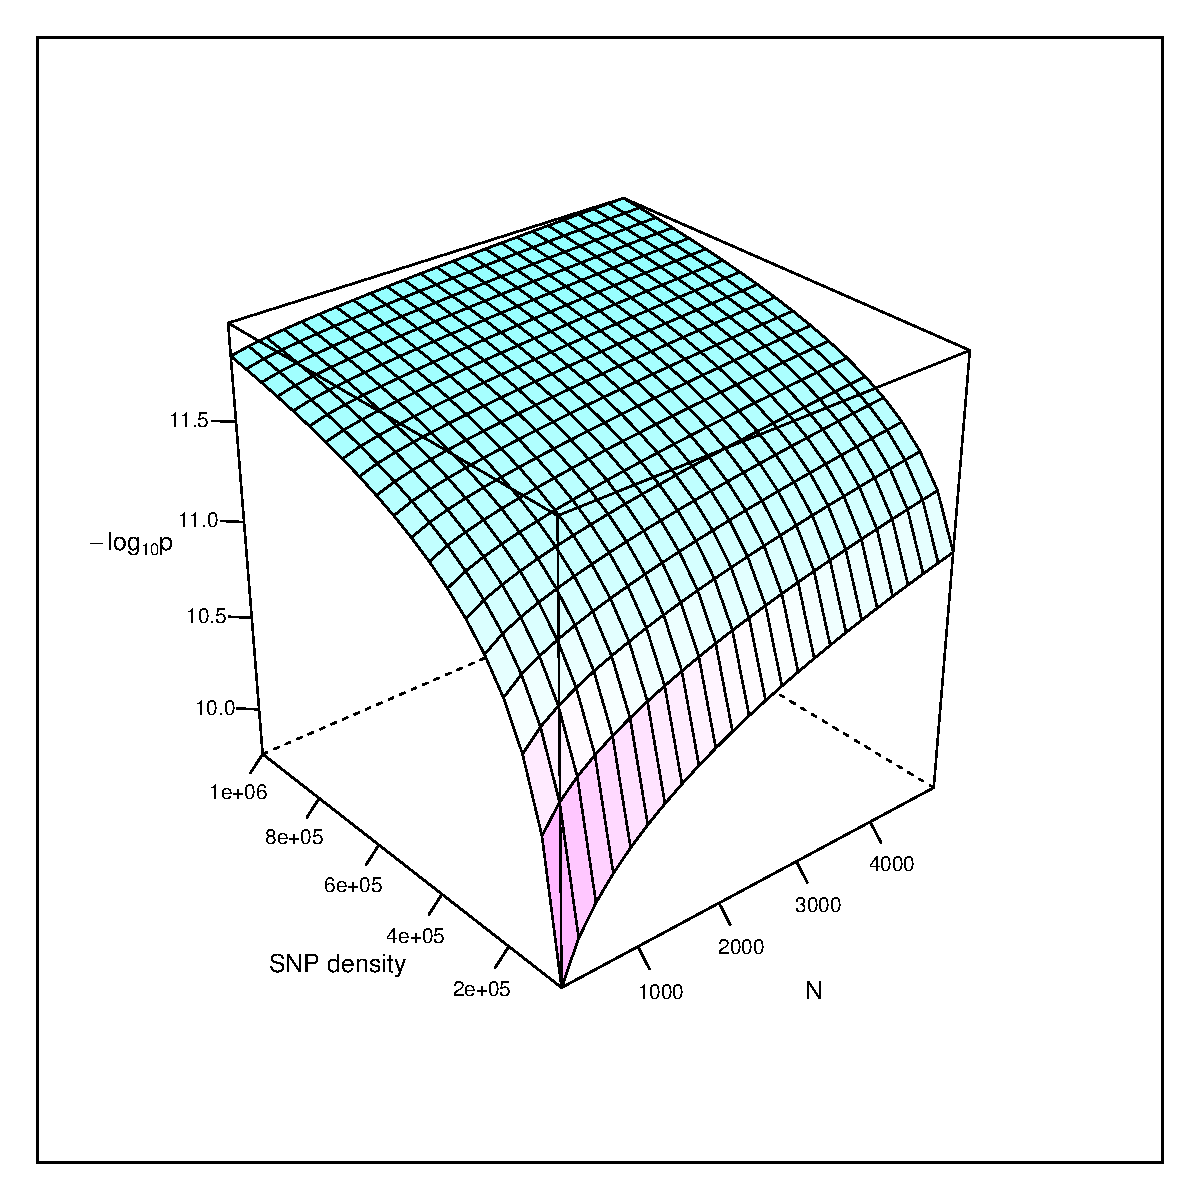
\includegraphics[height=7cm]{threshold_function.pdf}
	\end{center}
\end{frame}


\begin{frame}{More accurate thresholds?}
	\begin{itemize}
		\item 1641 complete scans were performed on permuted phenotype
		\begin{itemize}
			\item This means we can see how extreme the p-values would go by chance alone, because any real biological connection between genotype and phenotype has been severed, but the correlation structure remains intact
		\end{itemize}
		\item Threshold predicted to be: \textbf{11.648}
		\item Empirical estimate: \textbf{11.632}
		\item Average correlation between 5380 probes: \textbf{0.265}
		\item Estimate of threshold for all probes: $-\log_{10}p =$ \textbf{15.3}
	\end{itemize}
\end{frame}


\begin{frame}{Initial glance at the results}
	\begin{itemize}
		\item 71 probes have significant eQTLs after filtering for:
		\begin{itemize}
			\item Bonferroni threshold of 16.5
			\item Additive variance $\leq$ 60\% of total genetic variance
			\item Relatively common SNPs (must have samples for all 9 genotype classes)
			\item No LD between interacting SNPs
		\end{itemize}
	\end{itemize}
	\begin{block}{Overall:}
		Number of significant epistatic pairs after extremely conservative filtering: \textbf{140}!
	\end{block}
\end{frame}


\begin{frame}{Initial glance at the results}
	\begin{itemize}
		\item Proportion of the phenotypic variance explained:
	\begin{itemize}
		\item Total genetic: range 8.4\% - 17.1\%
		\item Total non-additive: range 3.5\% - 9.2\%
	\end{itemize}
		\item 14\% cis-cis
		\item 69\% cis-trans
		\item 17\% trans-trans
	\end{itemize}
\end{frame}


\begin{frame}{Some examples}
	\begin{center}
		\includegraphics[height=7.5cm]{epistasis_examples}
	\end{center}
\end{frame}


\begin{frame}{Next steps}
	\begin{itemize}
		\item Do they make biological sense?
		\item Replicate! We have a dataset with the same expression array
		\begin{itemize}
			\item Sample size is only 150, this will make things tricky!
		\end{itemize}
		\item Continue with the scan on remaining probes
		\begin{itemize}
			\item But unfortunately the cluster is currently being used by some astronomers...
		\end{itemize}
	\end{itemize}
\end{frame}



%%%%%%%%%%%%%%%%%%%%%%%%%%%%%%%%

\section*{}

\begin{frame}{Acknowledgements}

%%%%%%%%%%%%%%%%%%%%%%%%%%%%%%%%



	\begin{columns}[c]

		\column{.5\textwidth}
			{\tiny
				Compute resources
				\begin{itemize}
					\item ECDF - {\tt eddie}
					\item Daresbury Labs - {\tt cseht}
					\item IVEC - {\tt fornax}
					\item QBI cluster
				\end{itemize}
			}

		\column{.5\textwidth}
			{\tiny
				Complex Trait Genomics Group
				\begin{itemize}
					\item Peter Visscher
					\item Naomi Wray
					\item {\color{red} Joseph Powell}
					\item Jian Yang
					\item Allan Mcrae
					\item Anita Goldinger
					\item Hong Lee
					\item Anna Vinkhuyzen
					\item Guo-Bo Chen
					\item Beben Benyamin
					\item Zong Zhang
					\item Enda Byrne
					\item Marie-Jo Brion
					\item Sven Stringer
					\item Visit us at www.complextraitgenomics.com
				\end{itemize}
			}
		\end{columns}
\end{frame}


\begin{frame}
	\begin{columns}[ccc]
		\begin{column}{0.3\textwidth} \end{column}
		\begin{column}{0.3\textwidth}
			\centering
			\textbf{Thank you!}
		\end{column}
		\begin{column}{0.3\textwidth}\end{column}
	\end{columns}
\end{frame}


\begin{frame}{Sample size vs 2D threshold}


	\begin{equation}
		\lim_{n \to \infty} \bar{g} = 9 \nonumber
	\end{equation}

	\begin{eqnarray}
		-\log \left ( f \left (
		\frac{
			SS_{W}  (g - 1)^{-1}
		}{
			SS_{B} (n - g)^{-1}
		};
		g - 1, n - g
		\right ) \right )
		& \propto &
			n \nonumber \\ 
		& \propto &
			SS_{W} / (SS_{W} + SS_{B}) \nonumber \\
		& \propto & -\log(g)
		\nonumber
	\end{eqnarray}

\end{frame}



\begin{frame}{GP maps from genetic algorithm}
	\begin{center}
		\includegraphics[width=8cm]{gpmaps2.pdf}
	\end{center}
\end{frame}

\begin{frame}{Narrow-sense heritability}
	\begin{figure}
% \begin{minipage}[c]{0.38\textwidth}
		\includegraphics[width=6cm]{visscher2008_heritabiliy.jpg} \\
		{\tiny Visscher, 2008}
	\end{figure}
	\begin{itemize}
		\item Fitness related traits have lower heritabilites
		\item Additive variance appears to be maintained under selection
		\item Response to selection is lower than expected for fitness related traits
	\end{itemize}
\end{frame}


\begin{frame}{Allele frequency trajectories}
	\begin{center}
		\includegraphics[width=8cm]{allelefreq_det.png}
	\end{center}
\end{frame}

\begin{frame}{Changes in variance under selection}
	\begin{center}
		\includegraphics[width=10cm]{propadditive_det_grey.pdf} \\
		\includegraphics[width=10cm]{Vg_det_grey.pdf}
	\end{center}
\end{frame}

\begin{frame}{Power studies}
	\begin{center}
		\includegraphics[width=10cm]{powersimple.pdf} \\
	\end{center}
\end{frame}

\begin{frame}{Epistatic patterns}
	\begin{center}
		\includegraphics[width=8cm]{sup_gpmaps.pdf}
	\end{center}
\end{frame}

\begin{frame}{Allele frequency trajectories}
	\begin{center}
		\includegraphics[width=8cm]{sup_allelefreq_sim.png}
	\end{center}
\end{frame}

\begin{frame}{Detection is underpowered}
	\begin{center}
		\includegraphics[height=7.5cm]{gpmaps_ld.png}
	\end{center}
\end{frame}



\end{document}


